\documentclass[../main.tex]{subfiles}
\begin{document}

The first approach relies on the social-psychological model of Sawyer and Guetzkow. However, since it was not possible to trace the original book, about the model it is possible to say that it is based on five groups of variables intervening in a negotiation. They extrapolate a set of factors which play an important role within the context of a negotiation. Those factors are "contextual or situational, processual or behavioral, strategic or related to the outcome" \autocite[192]{faure}.

Faure asserts that culture is either embedded among contextual factors or acts through each analytical category.
To provide an explanation for this statement, Faure cites the book "U.S.-China Trade Negotiations" written by Rosalie Tung. In this book, she explains cultural influence by giving an insight on the negotiation between Chinese and American negotiators. Successively, Faure mentions an article written by Stephen Weiss: "Analysis of Complex Negotiations in International Business: The RBC Perspective". It explains the cultural influence on international negotiation through \textit{r}elationship, \textit{b}ehaviours, and influencing \textit{c}onditions (hence, the RBC perspective).\\

The book "U.S.-China Trade Negotiations" written by Tung is a vast analysis on the trade between American and Chinese companies. Particularly, a questionnaire was conducted on American firms, in order to identify the practices and procedures. For the purpose of this thesis, only the Chapter 3 of the book will be analysed, as it contains the analytical framework to contribute to this work.

The questionnaire had several sets of question concerning many topics. Specifically, information was gathered about: the history of the trade relationship on the American firm with China; the conduct of business negotiations; the degree of satisfaction or dissatisfaction of the company towards the negotiation; perceived differences in the decision-making approach between American and Chinese teams; negotiations' rate of success; the factors accountable for the success or the failure of negotiations; preparatory programs to help firm deal with negotiations; and operations' base to conduct trade with China \autocite[56]{tung}.

What is interesting for the scope of this chapter are the perceived differences in the decision-making process and the factors accounting for the success or the failure of the negotiations as these points deal with cultural factors.

\textbf{Decision-Making Styles}.
The set of question regarding this aspect generated mixed responses. Indeed, 26 percent of the respondents indicated that a member dominated the group decision; 21 percent suggested that no member of the group seem to have the power to make a decision; 18 percent reckoned that every team member had equal power in decision-making; the rest indicated that there was a leader in the team \autocite[63]{tung}.

The author provides us with two possible explanations for the mixed opinions. Either Americans think that they know how things work when they actually do not, or the fact that Chinese negotiators gather in a room to make decisions makes Americans unaware of the Chinese decision-making process.

Moreover, according to American respondents, Chinese negotiators take longer time to make a decision, focus more on a long-term relation, and are more indirect. This has to do with the different concept of time: indeed, Chinese cultures perceive time as cyclical and repetitive. Chinese have a longer view of time that lead them to take more time to make decisions. In addition, since Chinese are more inclined to the relationship among negotiators rather than to the issue itself, they will be more focused on the long-term period, rather than on the immediate present. Also, Chinese culture is defined high-context. It means that Chinese negotiators use indirect communication and disclose very little information if not at all\footnote{In the next chapter, there will be given detail analysis on the concept of time and on the dichotomy high-context/low-context cultures.}.

This opposition with American negotiators (who focus on the substantial issue and belong to a low-context culture) lead to a difference in the behaviour in the negotiation.

\textbf{Factors Responsible for Success or Failure of the Negotiations}. The questionnaire examines the factors perceived as successful or unsuccessful for a negotiation.

Concerning the successful factors, from the questionnaire's answers it was possible to identify three separate factors containing a total of eleven items \autocite[66]{tung}.

\textit{Attitude of US firms}. American negotiators reckon that the preparation of the American firms, the patience of US teams, the US team's sincerity, and the personal relationships were all elements of success (the preparation being the most successful one).

\textit{Product characteristic}. This factor included the uniqueness of the product, the need of Chinese people of American products, and the American technical expertise.

\textit{Familiarity with Chinese culture}. This factor (which is the most relevant for the purpose of this thesis) includes familiarity with "Chinese business practices, social customs, politics, and the language" \autocite[67]{tung}.

As far as it concerns the unsuccessful factors, by gathering the answers, it was possible to identify three factors that include a total of nine items.

\textit{Cultural differences}. This factor includes items such "differences in business practices, negotiation styles, social customs and culture, and communication breakdown" \autocite[67]{tung}. The cultural differences are indicated as the most relevant factor that leads to failure.

\textit{Product characteristic}. This factor is both success and failure related. However, the items characterising the factor are different. According to the responses of American negotiators, either Chinese did not really need the product that the firm was offering or there were too many competitors offering the same product.

\textit{Chinese insincerity}. As stated before, Chinese people belong to a high-context culture where communication is indirect and seldom negotiators disclose information about their interests. However, this factor was not considered as being relevant in the quest to find factors for the failure of negotiations (just 20 percent of the firms expressed the feeling of it being responsible "to a great extent").

It is possible to notice that culture is a key factor in both cases. In the successful factors, the familiarity of American negotiators with Chinese culture smoothen the process: however, this factor is necessary but insufficient for a negotiation to be successful.

In order to have a successful negotiation, Americans need to be willing to invest in a long-term relationship with Chinese negotiators by putting money, resources, and time in the process \autocite[71]{tung}.

Moreover, cultural differences are seen as an important difficulty in reaching a success. Cultural differences are perceived on many levels, and the author suggests that, in order to overcome the gap, American negotiators might document themselves through books or they can hire experts to train the negotiators \autocite[68]{tung}. Indeed, in order to negotiate with Chinese people, American negotiators should over come the cultural gap and embrace the issues and the intricacies \mancite\autocite[72]{tung}.

Cultural influence here is embedded in contextual factors as American and Chinese negotiate. When an American negotiator approaches a Chinese person to negotiate, it is like meeting someone in their own house: it is not sufficient to consider the personal culture within an individual, but their culture can be acknowledged and perceived also by a certain painting on the wall or by the disposition of the furniture. Everything counts.\\

Weiss article is relevant because of its perspective on the relationship among parties' relationship and behaviours and the influencing condition of a negotiation. Indeed, this perspective "is intended to be an inclusive, analytic perspective that furthers broad understanding of complex negotiations" \autocite[275]{weiss}.

The element that is significant for the purpose of this thesis is \textit{conditions}. As a matter of fact, conditions relate to those factors that stimulate or modify the parties' behaviours and relationships \autocite[286]{weiss}. However, in order to have a wider view on Weiss' work, also \textit{relationships} and \textit{behaviours} will be briefly analysed.

Before going into the RBC analysis, it is important to remark that Weiss also identifies three time period during which the negotiation happens: pre-negotiation, negotiation, and post-negotiation \autocite[289]{weiss}.
\textit{Pre-negotiation} starts when parties decide to negotiate with one another and ends when parties begin to make offers and counteroffers.
\textit{Negotiation} begins when parties set an agenda and they move from their respective initial positions and it ends when parties reach an agreement about the outcome of the process. \textit{Post-negotiation} begins right after and it does not have a designed endpoint.

Relationship, in the RBC perspective is conceived as the parties' "connectedness to each other as negotiators" \autocite[277]{weiss}. The focus is on the "space in between" the parties. This is important because a a negotiation concerns a relationship between the parties and because, at the end of a negotiation, if there is not an overarching relationship-based perspective, the final agreement of that negotiation will go unattended \mancite\autocite[277]{weiss}.

Weiss distinguishes three types of parties: primary, secondary, and third. The primary parties are the most directly involved in the negotiation. The secondary have an interest in the negotiation but are not directly involved. Third parties are the ones that do not play a regular role. The relationships (and behaviours) are considered to be among primary parties.
He also acknowledges three level of analysis: relationships among organisations, among groups, and among individuals \mancite\autocite[278]{weiss}.

Behaviours of primary parties are directed towards the other party or are affecting the counterpart in a negotiation. Both unintended behavioural effects and intentional negotiating actions are considered for the purpose of this analysis \autocite[279]{weiss}.
Moreover, Weiss identifies many spheres of action for the behaviours: other than the three he borrows from Colosi\footnote{See: Colosi, Thomas. “Negotiation in the Public and Private Sectors.” \textit{American Behavioral Scientist}, vol. 27, no. 2, 1983, pp. 229–253.}, he adds another three for a total of six behavioural areas:\\
1) \textit{Independent}: relevant to the negotiation but not communicated to the counterpart;\\
2) \textit{Horizontal}: directed at the counterpart at the negotiating table;\\
3) \textit{Internal}: happens within a party (e.g. the negotiating team);\\
4) \textit{Vertical}: happens between the party and their superior/subordinate;\\
5) \textit{Lateral}: happens between the party and their colleagues;\\
6) \textit{External}: directed to the outside of the negotiation (e.g. mass media). \mancite\autocite[286]{weiss}.

\begin{figure}[h]
    %\centering\includegraphics[width=0.8\textwidth]{images/cafoscari.png}
    \centering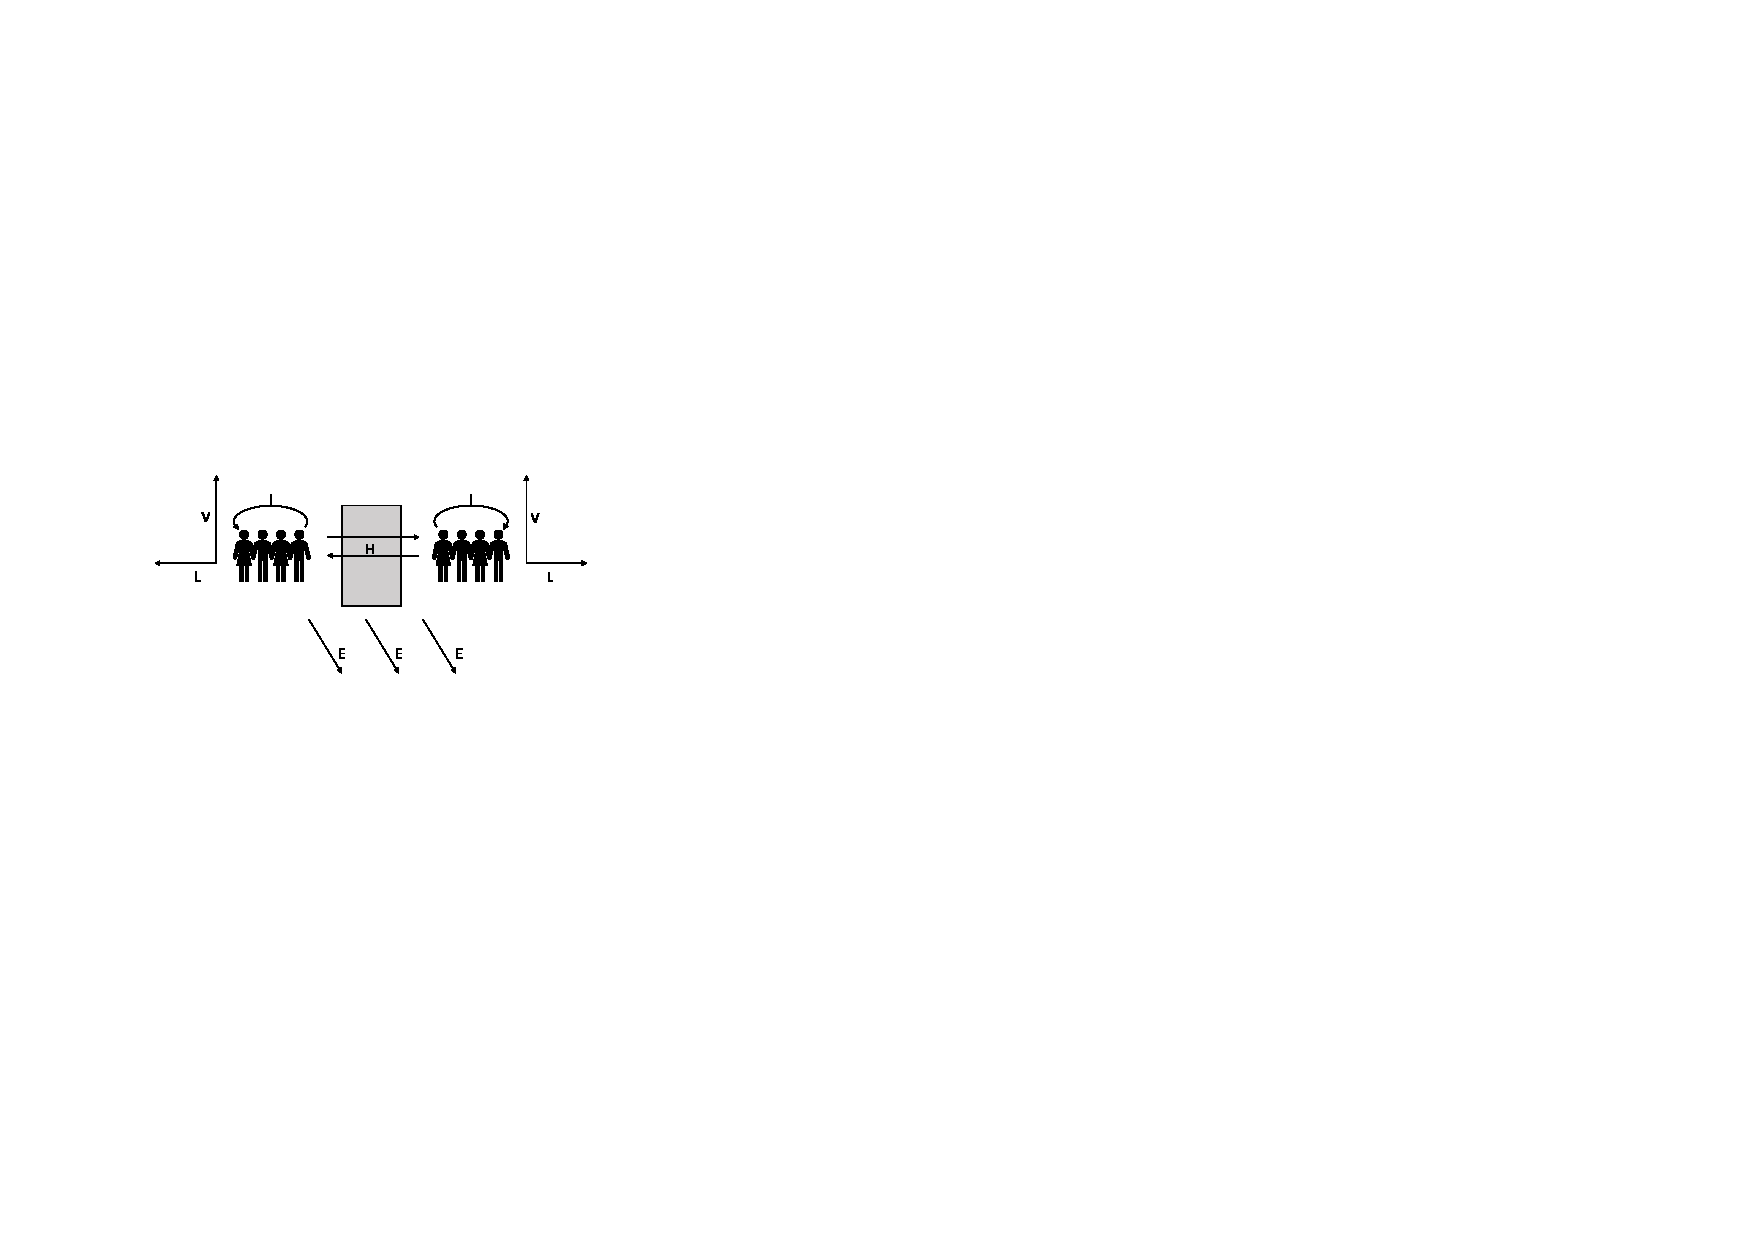
\includegraphics[width=0.7\textwidth]{images/weissss.pdf}
    \caption{Activities of the primary parties \autocite[286]{weiss}.}
\end{figure}

Weiss distinguishes four sets of conditions that have an influencing role within the negotiation process: circumstances, capabilities, cultures, and environments \autocite[287]{weiss}.
\begin{enumerate}
    \item \textit{Circumstances} refer to physical and social assets of the negotiation's context that address both parties. They include the availability of different communication channels, the media coverage, the presence of interpreters, just to cite some. These circumstances can influence the relationship and the behaviour of the parties at any level (individual, organisational, or group) \autocite[287]{weiss}.
    \item \textit{Capabilities} are the set of skills, resources, and traits of a primary party that make it capable of influence and be influenced by their counterpart, directly or indirectly, through behaviours. Capabilities include negotiating experience, personality, authority, and more \autocite[288]{weiss}.
    \item \textit{Cultures} refers both to the knowledge acquired by people to interpret the world to behave accordingly and to the set of learned behaviours \autocite[288]{weiss}\footnote{See also: Spradley, James P., and David W. McCurdy. \textit{Conformity and conflict: Readings in cultural anthropology}. Jill Potash, 2012. pg 2  and\\
    Gregory, Kathleen L. "Native-view paradigms: Multiple cultures and culture conflicts in organizations." \textit{Administrative science quarterly} (1983): 359-376.}.
    In complex negotiations, some cultural traits may be shared by both negotiating parties. Weiss classifies two cultural factors. First, both parties may form a "negotiator subculture". Second, the RBC view of general characteristics of a multicultural exchange depends on the awareness of the parties of those characteristics \mancite\autocite[289]{weiss}.
   \item \textit{Environments} refer to the sets of elements that are beyond the negotiation context but that somehow affect the parties' behaviour and relationships. Those elements include resources, power, legal frameworks, and, most importantly, other organisations 
\end{enumerate}

According to Weiss, cultural influence can be seen in all phases of the negotiation process. Indeed, in the pre-negotiation and negotiation phases, cultural influence can be perceived within the corporate culture of a negotiation, by looking for example at the information-sharing propensity; a cultural element can also be seen within the organisational control structure by looking at how and in which way the top management is involved in the negotiation or which communication channels are available. During the post-negotiation process, Weiss reckons that the main elements to be accounted in order to perceive a cultural influence are the corporate culture, the compensation of the negotiators, the national culture, and, once again, the organisational structure \mancite\autocite[285]{weiss}.

Moreover, Weiss adds that conditions influence the parties but the parties themselves can act in order to modify some conditions. Under this reasoning, "cultures not only influence parties' behaviour, but adapt and change because of it" \mancite\autocite[289]{weiss}.

Weiss work is visually reassumed in the following scheme.

\begin{figure}[h]
    %\centering\includegraphics[width=0.8\textwidth]{images/cafoscari.png}
    \centering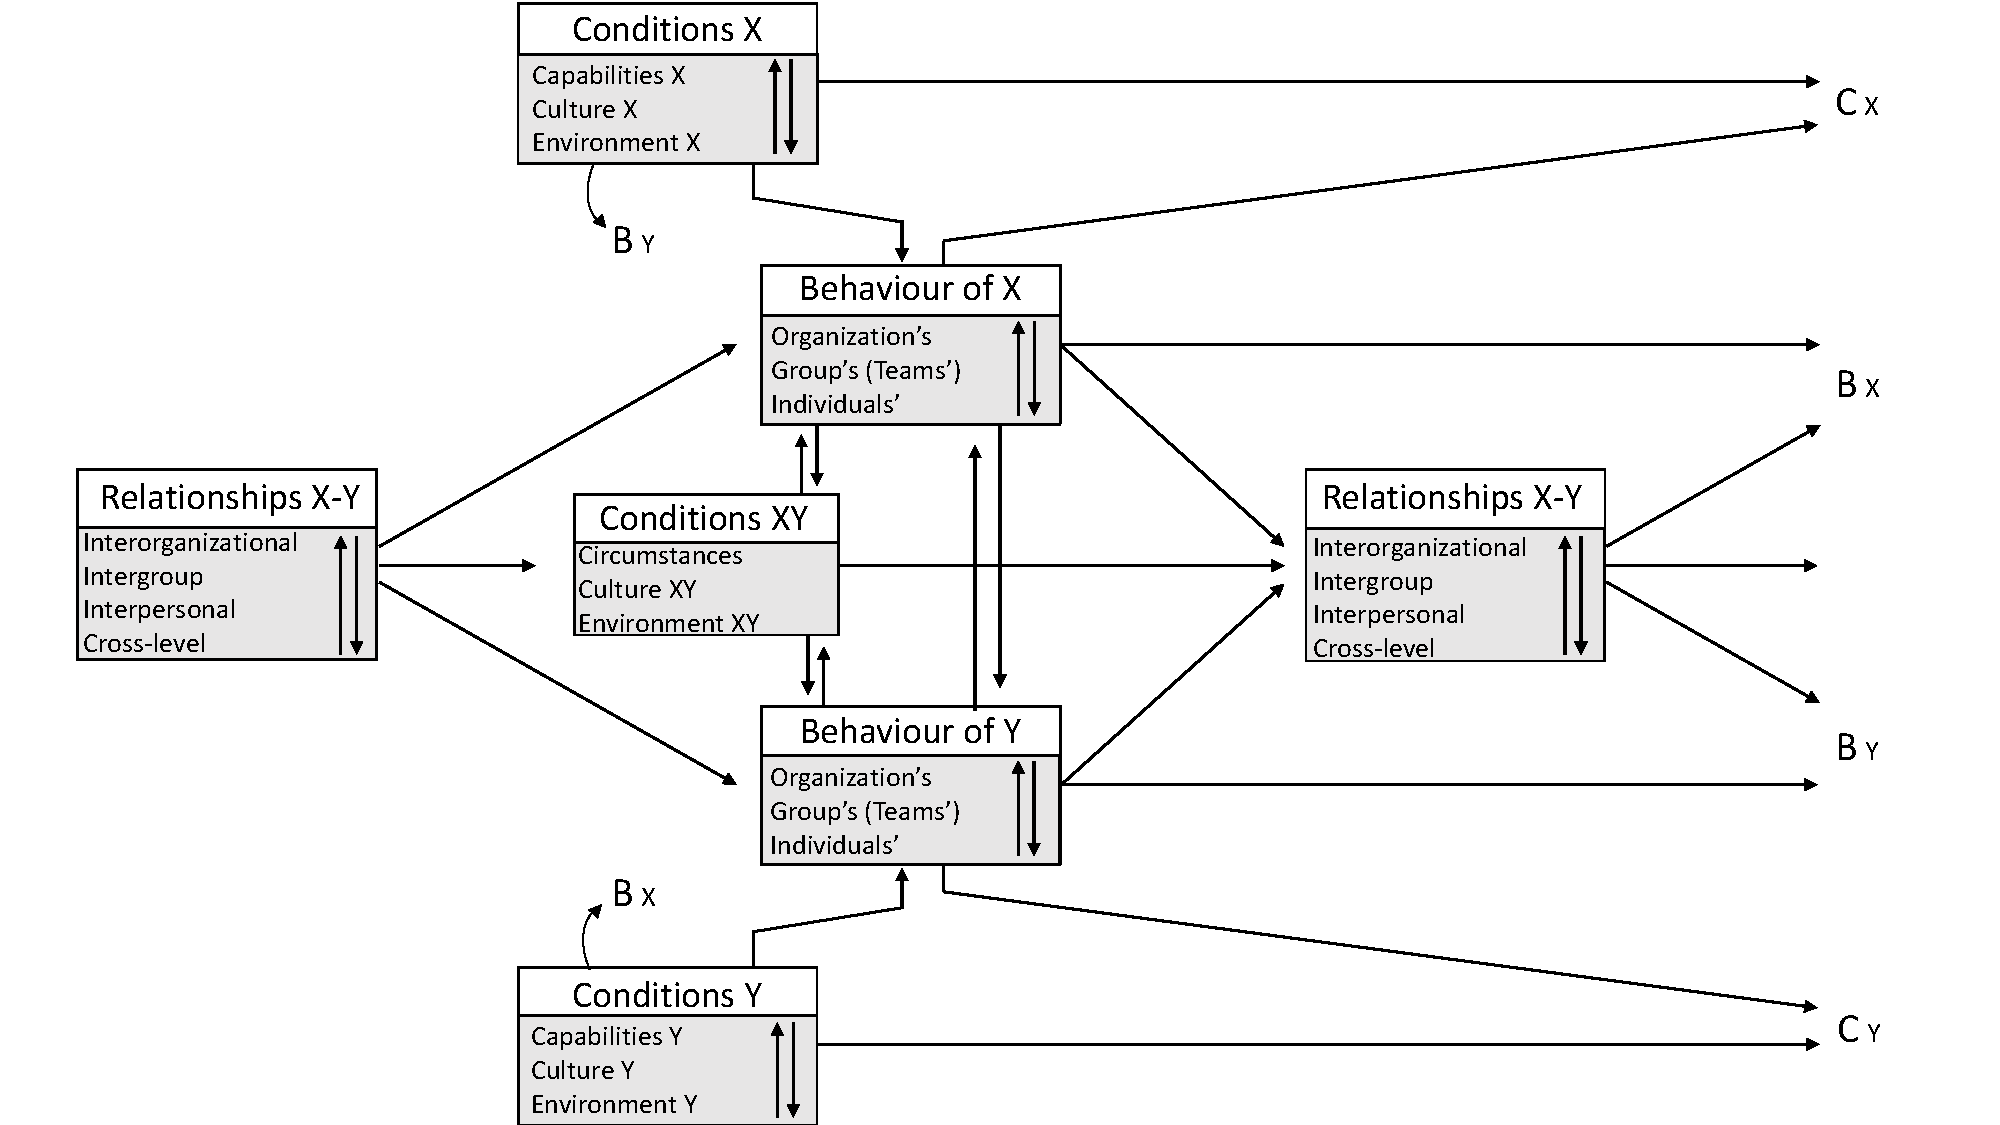
\includegraphics[width=\textwidth]{images/rbc.pdf}
    \caption{Basic RBC Model of a Complex Negotiation: X and Y are the parties negotiating.\mancite\autocite[276]{weiss}.}
\end{figure}\\

This approach in a way tells us that culture is already there, even before negotiators start a negotiation process. It is not manifested after parties begin to express themselves: it is contextual and it belongs to the factors that form the structural assets of a negotiation. In the next chapters, other approaches will be taken into consideration.


\end{document}